\documentclass[12pt]{article}

\usepackage[spanish]{babel}
\usepackage{hyperref}
\usepackage{graphicx}
\usepackage{listings}
\usepackage{color}
\usepackage{multicol}
\usepackage{amssymb}
\usepackage{enumitem}
\usepackage{here}
\usepackage{dsfont}
\usepackage{amsmath}
\usepackage{tipa}
\usepackage{float}
\spanishdecimal{.}

\title{Matemáticas para las Ciencias Aplicadas I}
\title{
	Cuarta Lista de Problemas \\
	\textbf{Primera  Parte} \\
	\vspace{1ex}
	\large Matemáticas para las Ciencias Aplicadas I \\
	Facultad de Ciencias, UNAM}

\date{\today}

\author{Flores Morán Julieta Melina \\ Zarco Romero José Antonio}

%% Sección 5.3: 44 y 73.
%% Sección 5.5: 28 y 37.
%% Sección 5.6: 58, 63 y 70.
%% Sección 5.8: 27.
%% Sección 5.9: 52 y 64

\begin{document}

\maketitle

%% 5.3 -----------------------------------------------------------------------------------------------------------------------------------------------------------------------------------------------------------------------------
\section{Sección 5.3 \\ Integración Por Sustitución}
% 44 -------------------------------------------------------------------------------------------------------------
\subsection{Ejercicio 44} name \\

Evaluar las integrales utilizando sustituciones apropiadas.
\[
\int \tan^3{5x}\sec^2{5x}dx
\]

% 73 -------------------------------------------------------------------------------------------------------------
\subsection{Ejercicio 73} name \\

\begin{enumerate}[label=(\alph*)]
\item Evalúe $\int [ x/\sqrt{x^2+1} ] dx$

\item Utilice una herramienta gráfica para generar algunas curvas integrales típicas de $f(x) = x / \sqrt{x^2 + 1}$ en el intervalo $(-5, 5)$.
  
\end{enumerate}

%% 5.5 -----------------------------------------------------------------------------------------------------------------------------------------------------------------------------------------------------------------------------
\section{Sección 5.5 \\ La Integral Definida}
% 28 -------------------------------------------------------------------------------------------------------------
\subsection{Ejercicio 28} name \\

Utilice el Teorema 5.5.4 y fórmulas apropiadas de geometría para evaluar las integrales.
\[
\int_{-3}^{0} \left(2+\sqrt{9-x^2}\right)dx
\]

% 37 -------------------------------------------------------------------------------------------------------------
\subsection{Ejercicio 37} name \\

Evaluar las integrales completando el cuadrado y aplicando fórmulas apropiadas de geometría.
\[
\int_{0}^{10} \sqrt{10x-x^2}dx
\]

%% 5.6 -----------------------------------------------------------------------------------------------------------------------------------------------------------------------------------------------------------------------------
\section{Sección 5.6 \\ El Teorema Fundamental Del Cálculo}
% 58 -------------------------------------------------------------------------------------------------------------
\subsection{Ejercicio 58} name \\

Defina $F (x)$ por
\[
F(x)=\int_{\pi/4}^{x} \cos{2t} dt
\]
\begin{enumerate}[label=(\alph*)]
\item Utilice la parte 2 del teorema fundamental del cálculo para encontrar $F'(x)$.
  
\item Verifique el resultado del inciso (a) integrando primero y luego diferenciando.
  
\end{enumerate}

% 63 -------------------------------------------------------------------------------------------------------------
\subsection{Ejercicio 63} name \\

Sea $F(x)=\int_{4}^{x} \sqrt{t^2+9}dt$. Encuentre
\begin{enumerate}[label=(\alph*)]
\item $F(4)$.
  
\item $F'(4)$.
  
\item $F''(4)$.
  
\end{enumerate}

% 70 -------------------------------------------------------------------------------------------------------------
\subsection{Ejercicio 70} name \\

Un ingeniero de tránsito monitorea la velocidad a la que los automóviles ingresan a la carretera principal durante la hora pico de la tarde. De sus datos estima que entre las 16.30 horas. y 5:30 p.m. la velocidad $R(t)$ a la que los automóviles ingresan a la carretera está dada por la fórmula $R(t) = 100(1 − 0.0001t^2 )$ automóviles por minuto, donde $t$ es el tiempo (en minutos) desde las 4:30 p.m.
\begin{enumerate}[label=(\alph*)]
\item ¿Cuándo ocurre el flujo máximo de tráfico hacia la carretera?
  
\item Estime el número de automóviles que entran a la carretera durante la hora pico.
  
\end{enumerate}

%% 5.8 -----------------------------------------------------------------------------------------------------------------------------------------------------------------------------------------------------------------------------
\section{Sección 5.8 \\ Valor Promedio De Una Función Y Sus Aplicaciones}
% 27 -------------------------------------------------------------------------------------------------------------
\subsection{Ejercicio 27} name \\

Un ingeniero de tránsito monitorea la velocidad a la que los automóviles ingresan a la carretera principal durante la hora pico de la tarde. De sus datos estima que entre las 16.30 horas. y 5:30 p.m. la velocidad $R(t)$ a la que los automóviles ingresan a la carretera está dada por la fórmula $R(t) = 100(1 − 0.0001t^2)$ automóviles por minuto, donde $t$ es el tiempo (en minutos) desde las 4:30 p.m. Encuentre la velocidad promedio, en automóviles por minuto, a la que los automóviles ingresan a la carretera durante la primera media hora de la hora pico.

%% 5.9 -----------------------------------------------------------------------------------------------------------------------------------------------------------------------------------------------------------------------------
\section{Sección 5.9 \\ Evaluación De Integrales Definidas Por Sustitución}
% 52 -------------------------------------------------------------------------------------------------------------
\subsection{Ejercicio 52} name \\

\begin{enumerate}[label=(\alph*)]
\item Utilice un CAS para encontrar el valor exacto de la integral
  \[
  \int_{-\pi/4}^{\pi/4} \tan^4{x} dx
  \]
\item Confirme el valor exacto mediante cálculo manual. [\textit{Sugerencia}: Utilice la identidad $1 + \tan^2{x}=\sec^2{x}$.]
\end{enumerate}

% 64 -------------------------------------------------------------------------------------------------------------
\subsection{Ejercicio 64} name \\

\begin{figure}[H]
\centering
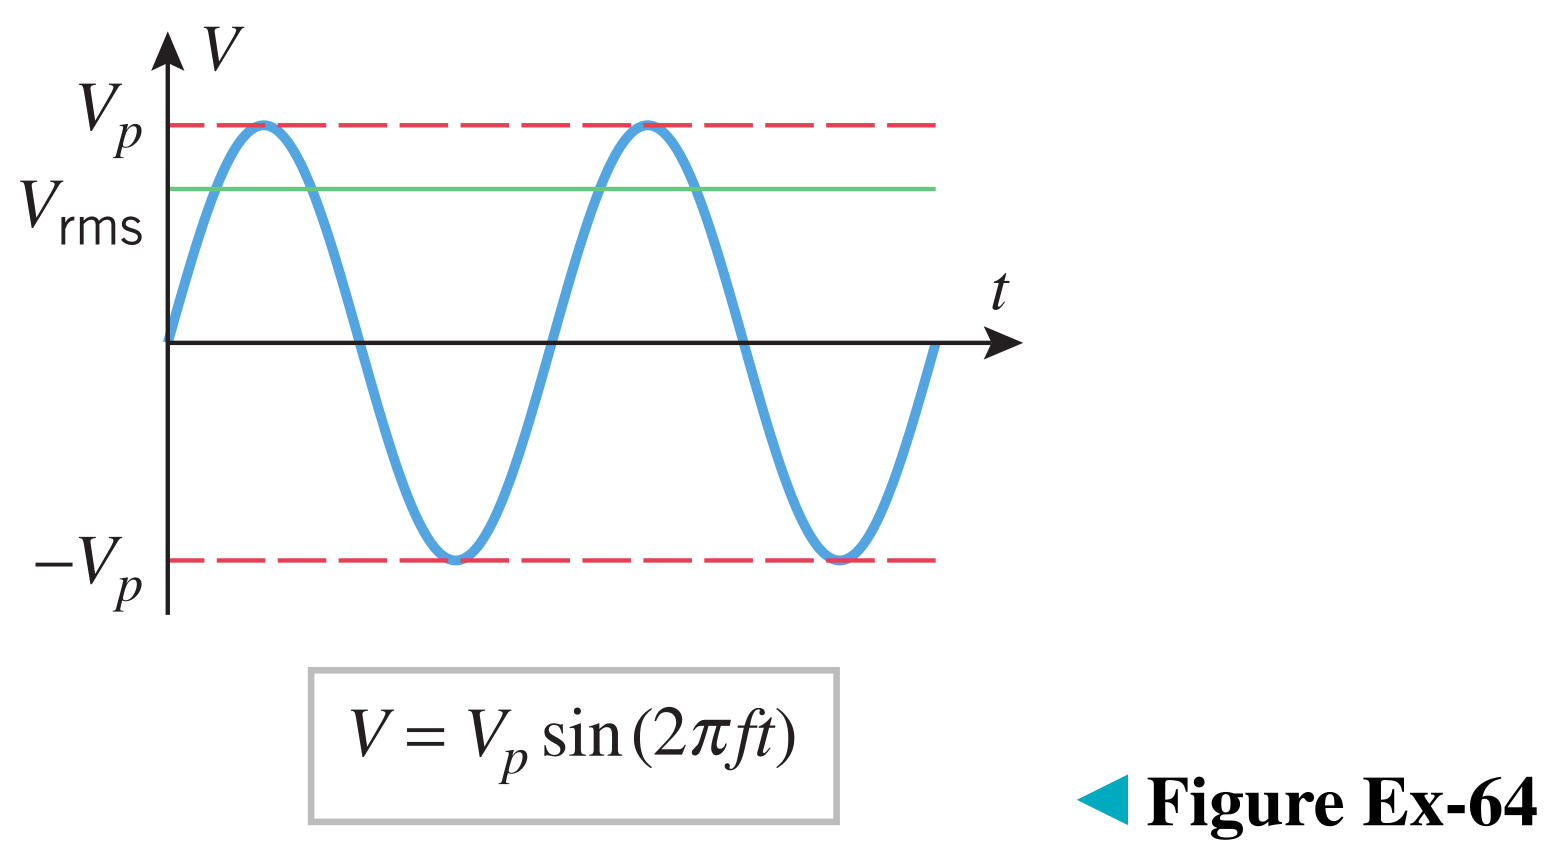
\includegraphics[width=0.7\textwidth]{../img/img_Lista4/1_64.png}
\end{figure}

La electricidad se suministra a los hogares en forma de \textbf{\textit{corriente alterna}}, lo que significa que el voltaje tiene una forma de onda sinusoidal descrita por una ecuación de la forma
\[
V = V_p \sin{(2\pi ft)}
\]
(ver la figura adjunta). En esta ecuación, $V_p$ se llama \textbf{\textit{voltaje máximo}} o \textbf{\textit{amplitud}} de la corriente, $f$ se llama \textbf{\textitfrecuencia}} y $1/f$ se llama \textbf{\textit{período}}. Los voltajes $V$ y $V_p$ se miden en voltios ($V$), el tiempo $t$ se mide en segundos ($s$) y la frecuencia se mide en hercios ($Hz$). ($1 Hz = 1$ ciclo por segundo; un \textbf{\textit{ciclo}} es el término eléctrico para un período de la forma de onda). La mayoría de los voltímetros de corriente alterna leen lo que se llama \textbf{\textit{rms}} o \textbf{\textit{valor cuadrático medio}} de $V$. Por definición, ésta es la raíz cuadrada del valor promedio de $V^2$ durante un período.
\begin{enumerate}[label=(\alph*)]
\item Demuestre que
  \[
  V_{rms}=\frac{V_p}{\sqrt{2}}
  \]
    [\textit{Sugerencia}: Calcule el promedio durante el ciclo de $t= 0$ a $t = 1/f$ y use la identidad $\sin^2{\theta}= \frac{1}{2}(1-\cos{2\theta})$ para ayudar a evaluar la integral.]
  
\item En Estados Unidos, los enchufes eléctricos suministran corriente alterna con un voltaje $rms$ de $120 V$ a una frecuencia de $60 Hz$. ¿Cuál es el voltaje máximo en tal tomacorriente?

\end{document}
